%!TEX root = ../stoeter_sourcecount.tex
\section{DNNs for Count Estimation}%
\label{sec:supervised_learning}
% A short review of deep learning architectures used for related tasks and proposal for count estimate architectures.
Applying deep learning to an existing task, often is a matter of choosing a suitable network architecture.
Typically an architecture describes the overall structure of the network including (but not limited to) the type and number of layers in the network and how these layers are connected to each other.
In turn, designing such an architecture requires deep knowledge about input and output representations and their required level of abstraction.
% Introduce our three/five basic networks. For all of them we:
% * reference the use cases, and the strengths and weaknesses,
% * explain why and how they can be used for count estimation
Many audio related applications like speech recognition~\cite{HintonSpeech} or speaker diarization share similar common architectural structures, often found by incorporating domain knowledge and through extensive hyper parameter searches.
For our task of source count estimation, however, domain knowledge is difficult to incorporate, as our studies aim at revealing the best strategy to address the problem.
This is why we chose architectures that already have shown a good level of generalizability for audio applications.
All architectures under investigation are summarized in Figure~\ref{fig:networkoverview}.
\par
% introduce some basic notations for the input
The input of all networks is a batch of samples, represented as time frequency representations \(\mathbf{X} \in \mathbb{R}^{ D \times F \times C } \), where \(D\) refers to the time dimension, \(F\) to the frequency dimension and \(C\) to the channel dimension (in the single-channel case, \(C=1\)).
In the following, we discuss several commonly used DNN architectures and their benefits in using them for the task of estimating the number of speakers.


\subsubsection{Convolutional Neural Network (CNN)}%
Convolutional Neural Networks (CNNs) are a variant of standard fully-connected neural networks, where the architecture generally consists of one or more ``convolution layers'' followed by fully-connected layers leading to the output.

A convolution layer generally consists of a convolution operation, followed by feature pooling.
The convolution operation applies a set of filters to local regions of the input, and the application of each such filter outputs a \emph{feature map}.
It should be noted that the convolution operation, generally, also constitutes the application of a point-wise non-linear activation function on each feature map.
This is followed by feature pooling, that aims to reduce the feature space dimensions by combining the filter activations over a specified region.
Since the individual elements of the filters (weights) are learned during the training stage, convolution layers can also be interpreted as feature extractors.
By stacking up additional layers, CNNs can extract more abstract features in higher level layers~\cite{Simonyan15}.
\par
The sizes of the filter kernels are crucial, and it was shown in~\cite{pons2017timbre} that many audio applications can benefit if domain knowledge is put into the design of the filter kernel size.
The use of small filter kernels, as often used in image classification tasks, does not necessarily decrease performance, when combined with many layers.
Also larger kernels increase the number of parameters and therefore the computational complexity.
It was shown in~\cite{schluter15} that \(3 \times 3\) kernels resulted in state-of-the-art results in singing voice detection tasks.
Due to its hierarchical architecture, CNNs with small filters have the benefit that they can model time and frequency invariances regardless of the scaling of the frequency axis.
\par
Our proposed architecture is similar to the ones proposed by ~\cite{schluter16} used for singing voice activity detection.
In our proposed CNN, we consider local filters of size \(3 \times 3\). In the first layer, 2D convolution is performed by moving the filter across both dimensions of the input in steps of 1 element (striding \(s = 1\) to generate \(C = 64\) feature maps/channels resulting in an output volume of \(64 \times (D - 3 + 1) \times (F - 3 + 1)\).
In the subsequent convolution layers, a similar operation is applied but for each convolutional layer, we consider a different number of feature maps.
Note, that the convolution operation is performed independently for every input channel, and then summed up along the dimension \(C\) for each output element.
In preliminary experiments we found that by using max-pooling we received significantly better performance when used after CNN layers.

\subsubsection{Recurrent Neural Network (RNN)}%
While convolutional layers excel in capturing local structures, RNNs can detect structure in sequential data of arbitrary length.
This makes it ideal to model time series, however, in practice, the learned temporal context is limited to only a few time instances, because of the vanishing gradient problem~\cite{Hochreiter98}.
To alleviate this problem, forgetting factors (also called gating) were proposed.
One of the most popular variants of RNNs with forgetting factors is the Long Short-Term Memory (LSTM)~\cite{Hochreiter97} cell.
In~\cite{stoeter17} such an architecture based on three bi-directional LSTM cells, was proposed. The architecture is similar to the one employed in~\cite{Leglaive15}.

% \begin{figure}[t]
% \centering
% 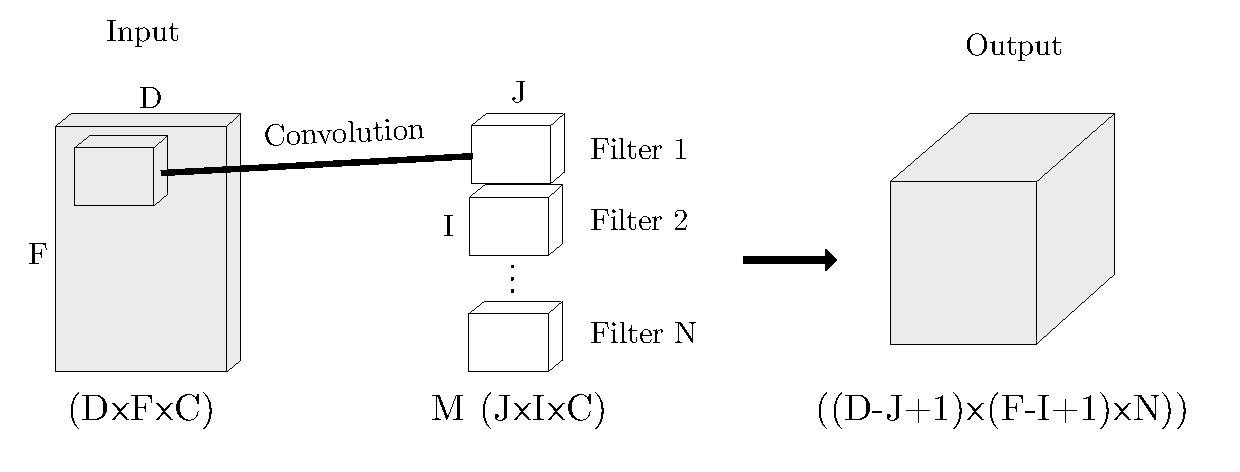
\includegraphics[width=\columnwidth]{figures/conv.pdf}
% \caption{Illustrative diagram to show the convolution operation in
% convolution layers of CNN.\@ We consider N different local filters each
% of size \(J\times I\)}%
% \label{fig:conv}
% \end{figure}

% * good for temporal dependencies.
% * State-of-the-art speech recognition, NLP, diarization
% A recurrent neural network (RNN) layer is very similar to a fully connected network, except that RNN applies the same set of weights \(\mathbf{A}\) recursively over an input sequence.
% While convolutional layers excel in capturing local structures, RNNs can detect structure in sequential data of arbitrary length. %have an internal memory of infinite length of the past input sequence history.
% This makes it ideal to model time series, however, in practice, the temporal context learnt is limited to only a few time instances, because of the vanishing gradient problem~\cite{Hochreiter98}.
%
% To alleviate this problem, forgetting factors (also called gating) were proposed.
% One of the most popular gated recurrent cells is the Long Short-Term Memory (LSTM)~\cite{Hochreiter97} cell.
% Its effectiveness has been proven in various applications and LSTMs are the state-of-the-art approach for speech recognition~\cite{Graves13} and singing voice detection~\cite{Leglaive15}~\footnote{For a deeper mathematical background of LSTMs, due to space constraints, the reader is referred to the aforementioned papers.}.
% For a given input of dimensions \(D \times F \times C\), the output of a recurrent layer is either only the last step of dimension \(1 \times A\) or the full sequence \(D \times A\).
% The latter is useful to stack multiple LSTMs or to apply temporal max pooling of the sequence.

\subsubsection{Convolutional Recurrent Neural Network (CRNN)}%
% * Combination of CNN and Recurrent
Recently the a combination of convolutional and recurrent (LSTM) layers were proposed for audio related tasks~\cite{sainath15, amodei16, Choi17, cakir17}.

The main motivation to stack these layers is to combine the benefits of convolutional layers with those of recurrent architectures, namely the benefit of convolutional layers in aggregating local features with the ability of recurrent layers to model long-term temporal data.

There are different ways to stack CNNs and RNNs to form a CRNN architecture.
In our application the motivation is to aggregate local time-frequency features coming from the output convolutional neural network and use the LSTM layer to model long temporal structures.
As the output of a CNN layer is a 3D volume \(D \times F \times C\) and the input of a recurrent layer only takes a 2D sequence, the dimension would need to be reduced. Naturally, the time dimension would need to be kept, therefore the channel dimension \(C\) is stacked with the frequency dimension \(F\) resulting in a \(D \times F \cdot C\) output.
% \begin{figure}[t]
% \centering
% 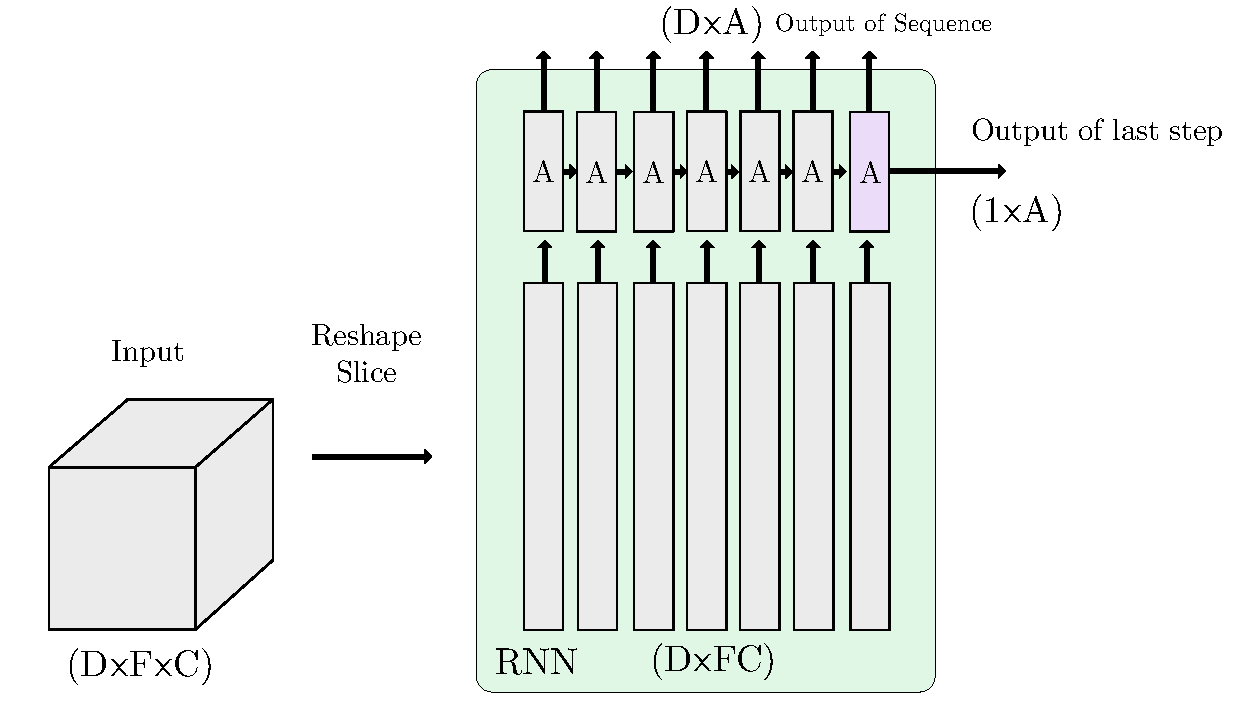
\includegraphics[width=\columnwidth]{figures/crnn.pdf}
% \caption{Illustrative diagram to show the stacking of the output of a convolution layer into a recurrent layer with \(A\) hidden nodes per memory cell.}%
% \label{fig:crnn}
% \end{figure}

\subsubsection{Full-band Convolutional Neural Networks (F-CNN)}%
% * using full frequency band filters.
% * Very few Parameters, easy to train.
Architectures where filters span the full frequency range and therefore apply convolution in temporal direction only, have already been successfully deployed in speech~\cite{amodei16} and music application~\cite{Choi17, Pons16, Dieleman14}).
Our motivation here is that the activity of speakers happen over wide frequency ranges and a count (unlike in counting objects in images) cannot be split into sub counts.
The full-range kernel configuration only affects the first hidden layer, as in consecutive outputs all frequency bands are squashed down to one single frequency band using ``valid'' convolutions.
This is computationally very efficient, because it reduces the middle layer's dimensionality of the network significantly due to this aggregation.
To further optimize the performance of the network, we applied a hyper parameter optimization technique using Tree-structured Parzen Estimator (TPE)~\cite{bergstra11}.
We used a search space of several hyper parameters as shown in Table~\ref{tab:fcnnhyper} and set the maximum number of evaluations to 200.

\begin{table}
  \caption{Parameter Optimization of F-CNN Model through hyper-parameter search. Bold hyper-parameters were found optimal.}%
  \label{tab:fcnnhyper}
  \centering
\begin{tabular}{lll}
  \toprule
  Layer               & Parameters        & Value Range \\
  CNN 1               & Feature Maps      & \( \{16, \mathbf{32}, 64\} \) \\
  CNN 1               & Filter Length     & \( \{\mathbf{3}, 5, 7\} \) \\
  Pooling 1           & Pooling Length    & \( \{1, \mathbf{2}, 4\} \) \\
  CNN2                & Feature Maps      & \( \{16, \mathbf{32}, 64\} \) \\
  CNN2                & Filter Length     & \( \{\mathbf{3}, 5, 7\} \) \\
  Pooling 2           & Pooling Length    & \( \{1, 2, 4\} \) \\
  \midrule
  CNN 3               & Presence of Layer & \( \{\mathbf{Yes}, No\} \) \\
  CNN 3               & Feature Maps      & \( \{16, 32, \mathbf{64}, 128\} \) \\
  CNN 3               & Filter Length     & \( \{\mathbf{3}, 5, 7\} \) \\
  Pooling 3           & Pooling Length    & \( \{1, \mathbf{2}, 4\} \) \\
  \midrule
  Fully Connected 1   & Hidden Unit       & \( \{64, \mathbf{128}\} \) \\
  Dropout 1           & Dropout Percentage& \( [0.1, \mathbf{0.2}, 0.5] \) \\
  Fully Connected 2   & Hidden Unit       & \( \{32, \mathbf{48}\} \) \\
  Dropout 2           & Dropout Percentage& \( [0.1, \mathbf{0.2}, 0.5] \) \\
  \bottomrule
  \end{tabular}
\end{table}

The results are in agreement with the findings in~\cite{schluter16} where small filter kernels of size 3 outperformed larger kernels. Also it can be seen from the results, that increasing the number of feature maps of the convolutional layers does not necessarily increase the performance.

\subsubsection{Full-Range Convolutional Recurrent Neural Networks (F-CRNN)}%
% * Also add recurrent.
Similarly to \emph{CRNN} and to the Deep Speech 2 implementation~\cite{amodei16}, we added an LSTM recurrent layer to the output of the last convolutional layer.
Since each filter output is only of dimension one, an additional flattening as in \emph{CRNN} is not required.

% \subsection{Output Activation Functions for Count Estimation}%
% \label{ssec:objectives}
% As we introduced in Section~\ref{ssec:estimation_framework}, the count estimation problem can be addressed using three different strategies.
% For each of the decision function a suitable output activation and loss is used.
%
% % Reference image object counting networks.
% % * Describe matching loss functions in detail.
% % Describe the DNN networks output layers very shortly
%
% % * Classification+Softmax
% \subsubsection{Classification}
% For \emph{classification}, the output is required to be one-hot-encoded so that the output is of dimension \(y \in \mathbb{B}^{L + 1}\), where \(L\) is the maximum number of concurrent speakers to be expected.
% In the final layer of the network, a softmax activation
% function is used to perform classification:
% \begin{equation}
%   f_j(z) = \frac{e^{z_j}}{\sum_k e^{z_k}}
% \end{equation}
% The softmax activation function generates the posterior probability for each of the \(L + 1\) classes, by squashing the output of the last layer to values between 0 and 1.
% The categorical cross entropy is used to generate the loss where \(p\) is the correct probability and \(u\) is the amount generated by model:
%
% \begin{equation}
%   E = \sum p(x) \log(u)
% \end{equation}
%
% % * Regression+MSE
% \subsubsection{Gaussian Regression}
% For the gaussian regression model the final output layer is of dimension \(y \in \mathbb{R}^{1}\).
% An activation function is not applied, the output is therefore linear.
% For training we use the mean squared error (MSE) function
%
% \begin{equation}
%   E = \sum \left|k-u\right|^{2}
% \end{equation}.
%
% Using the MSE can be interpreted as being derived from the negative log likelihood of normal distribution.
% So when we use MSE, we estimate the mean parameter of Normal distribution (output of the model) that is most likely to generate our data.
%
% % * Regression+Poisson Loss
% \subsubsection{Poission Regression}
% Poisson loss calculates the likelihood of parameter \(\lambda \) given the true count \(\cardinality \) using the negative log likelihood loss (also poisson loss):
%
% \begin{equation}
%   E = \sum \lambda - \cardinality * \log(\lambda + eps)
% \end{equation}.
%
\begin{figure*}[tb]
\centering
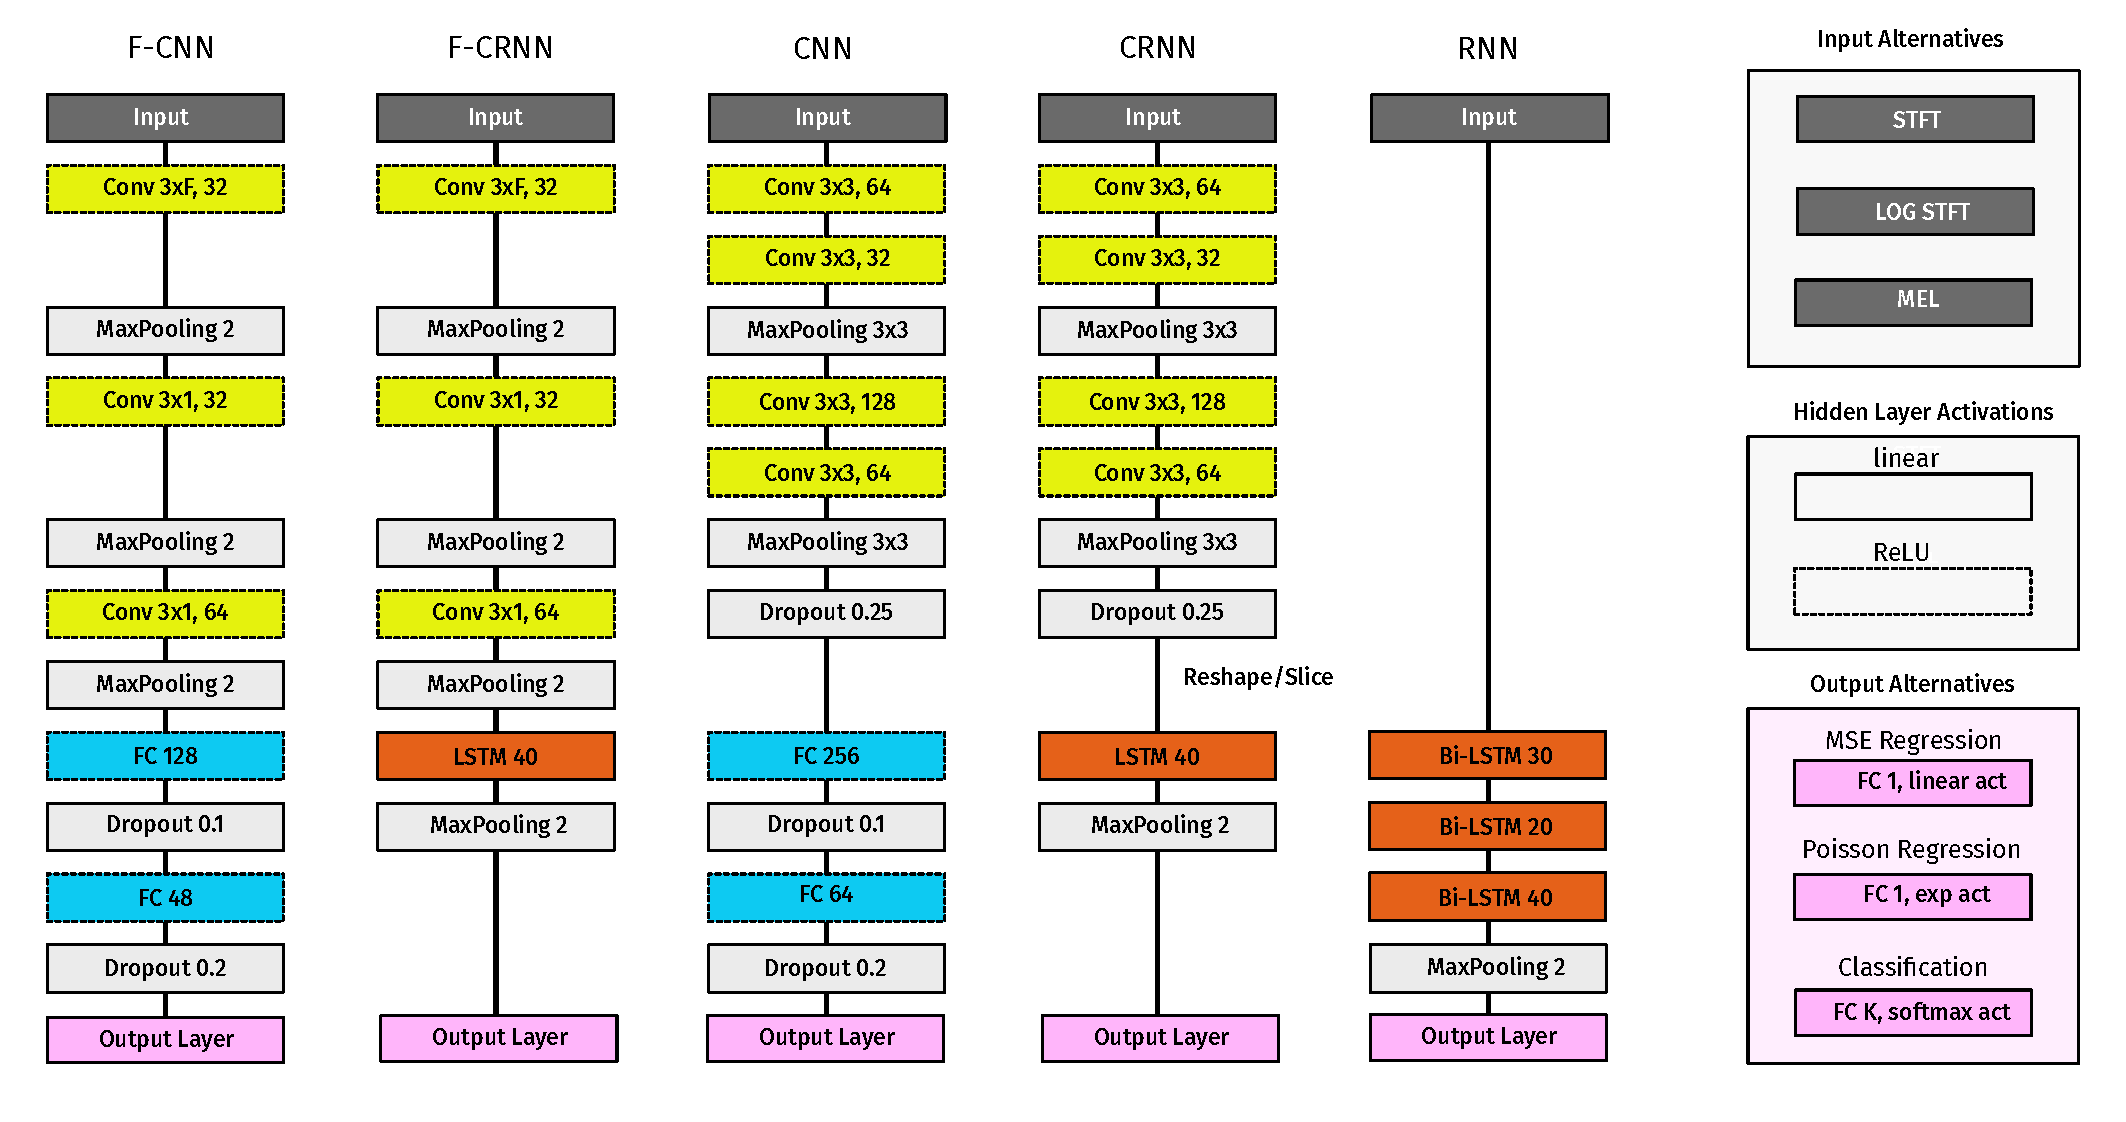
\includegraphics[width=0.9\textwidth]{Chapters/08_Analysis_CountNet/dsc/figures/networkoverview.pdf}
\caption{Overview of the proposed Architectures.}%
\label{fig:networkoverview}%
\end{figure*}
